\paragraph{L'énumération NetworkState}

\begin{minipage}
    {\linewidth}
    \centering
    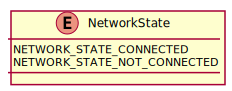
\includegraphics[width=0.5\linewidth]{../schemas/Conception_detaillee/enum_NetworkState.pdf}
    \captionof{figure}{Diagramme de l'énumération NetworkState}
\end{minipage}

\subparagraph{Philosophie de conception \newline} 

\medspace

L'énumération NetworkState a été définie précédemment, ici, les énumérations seront uniquement listées. 

\subparagraph{Description structurelle \newline}

\medspace

\textbf{Attributs :}

N.A.

\textbf{Services offerts :}

\begin{itemize}
    \item NETWORK\_STATE\_CONNECTED
    \item NETWORK\_STATE\_NOT\_CONNECTED
\end{itemize}